% Provenance (never printed): see sources/outline_sources.md (Year 3:
% spectral signatures; optical, thermal and radar sensors; radar
% interferometry; digital elevation models; GIS operations).
% Brief: sources/book5/BRIEFS.md, ch. 25. Curves from figdata/bachelor-3/
% spectral_signatures.py (ECOSTRESS spectra and the Landsat 8 OLI bands),
% thermal_ir.py (Planck's law, brightness temperatures, a mixed pixel),
% insar_mogi.py (the wrapped interferogram of a Mogi source) and
% varden_gis.py (slope, aspect and an overlay on the Varden Hills, from
% figdata/shared/region.py, read only). Exercise and problem values in the
% Book 5 scratch calculator calc/ch25.py. Mount Halvren, its lava flows and
% its fumaroles are invented. The brief's overlay (slope > 15 degrees on
% limestone within 200 m of the river) is empty on the Varden model: the
% valley floor is flat; the printed overlay uses the shale within 1 km.
\chapter{Teledetectie en GIS}\label{ch:b3:remote-sensing-gis}

In 1997 begon de grond van een wildernis in de Cascade Range, nabij het
vulkaancomplex dat de Three Sisters heet, te stijgen. In 2001 stond het midden ervan
\qty{15}{cm} hoger. Er staat geen vulkaan recht boven de zwelling, en de
laatste uitbarsting in het gebied was 1\,500 jaar oud. De opheffing werd door niemand
gevonden die er overheen liep: ze verscheen als een schietschijf van gekleurde ringen
toen radarbeelden van de regio, die van jaren na elkaar vanuit een baan waren genomen,
werden samengevoegd. De ringen plaatsten het binnendringende magma op 6 tot
\qty{7}{km} diepte; in maart 2004 trof een zwerm van meer dan 300 kleine aardbevingen
vlak naast hun middelpunt. Dit hoofdstuk legt uit hoe een satelliet een verandering van
enkele centimeter meet vanaf honderden kilometers hoogte, wat de andere sensoren in een
baan van de grond zien, en hoe de kaarten die zij maken in een
geografisch informatiesysteem worden samengevoegd.
% ledger: usgs:insar-fs

\begin{recall}
Het elektromagnetisch spectrum, de wet van Planck voor het zwarte lichaam,
emissiviteit en de wet van Kirchhoff, reflectie en de interferentie van golven
staan in de natuurkundeboeken. Teledetectie, satellietbeelden, kaartprojecties
en satellietpositiebepaling staan in de schoolboeken. Atmosferische vensters en
fotometrische banden staan in Boek~3, in het hoofdstuk over telescopen;
het digitale hoogtemodel en het geografische informatiesysteem dat het opslaat,
in het hoofdstuk over geologische kaarten; de eerste radarkaart van de
verplaatsing door een aardbeving, in het hoofdstuk over de aardbevingsbron. De
Mogi-bron van een zwellend magmareservoir staat in Boek~4, in het hoofdstuk
over vulkaanuitbarstingen.
\end{recall}

\section{Spectrale signaturen en optische sensoren}\label{sec:b3:remote-sensing-gis:optical}

Zonlicht dat de grond bereikt, wordt deels geabsorbeerd en deels
gereflecteerd, in verhoudingen die afhangen van de golflengte en van de stof waaruit de grond bestaat.
Een sensor in een baan meet het gereflecteerde licht in enkele
golflengtebereiken, zijn banden, en de verhoudingen tussen de banden
identificeren het oppervlak.

\begin{definition}[Spectrale signatuur]\label{def:b3:remote-sensing-gis:signature}
De \emph{spectrale signatuur}\index{spectrale signatuur} van een materiaal is
zijn reflectie als functie van de golflengte, $R(\lambda)$, de fractie van de
invallende straling die het reflecteert. Over het thermische infrarood, waar
oppervlakken eerder uitzenden dan reflecteren, is de signatuur de
emissiviteit $\varepsilon(\lambda)$; voor een ondoorzichtig monster geldt $\varepsilon = 1 - R$.
\end{definition}

\begin{omfigure}
\centering
\begin{tikzpicture}
\begin{axis}[width=0.9\linewidth, height=6.4cm, xmin=0.4, xmax=2.5, ymin=0, ymax=1,
  xlabel={golflengte (\unit{\micro\metre})}, ylabel={reflectie},
  tick label style={font=\scriptsize}, label style={font=\small},
  legend style={font=\scriptsize, at={(0.5,-0.24)}, anchor=north, /tikz/every even column/.append style={column sep=4pt}},
  legend columns=5, clip=false]
\fill[black!8] (axis cs:0.45,0) rectangle (axis cs:0.51,1);
\fill[black!8] (axis cs:0.53,0) rectangle (axis cs:0.59,1);
\fill[black!8] (axis cs:0.64,0) rectangle (axis cs:0.67,1);
\fill[black!8] (axis cs:0.85,0) rectangle (axis cs:0.88,1);
\fill[black!8] (axis cs:1.57,0) rectangle (axis cs:1.65,1);
\fill[black!8] (axis cs:2.11,0) rectangle (axis cs:2.29,1);
\addplot[very thick, green!50!black] table[x=um, y=grass] {figdata/out/bachelor-3-spectral_signatures-spectra.dat};
\addlegendentry{groen gras}
\addplot[thick, brown!70!black, dashed] table[x=um, y=soil] {figdata/out/bachelor-3-spectral_signatures-spectra.dat};
\addlegendentry{bruine zandgrond}
\addplot[thick, black!55] table[x=um, y=kaol] {figdata/out/bachelor-3-spectral_signatures-spectra.dat};
\addlegendentry{kaoliniet}
\addplot[thick, red!70!black, dash dot] table[x=um, y=hem] {figdata/out/bachelor-3-spectral_signatures-spectra.dat};
\addlegendentry{hematiet}
\addplot[thick, omDef] table[x=um, y=water] {figdata/out/bachelor-3-spectral_signatures-spectra.dat};
\addlegendentry{water}
\node[font=\tiny, anchor=south] at (axis cs:0.48,1) {2};
\node[font=\tiny, anchor=south] at (axis cs:0.56,1) {3};
\node[font=\tiny, anchor=south] at (axis cs:0.655,1) {4};
\node[font=\tiny, anchor=south] at (axis cs:0.865,1) {5};
\node[font=\tiny, anchor=south] at (axis cs:1.61,1) {6};
\node[font=\tiny, anchor=south] at (axis cs:2.2,1) {7};
\end{axis}
\end{tikzpicture}
\par\smallskip{\small Laboratoriumreflectiespectra van vijf oppervlakken (ECOSTRESS
Spectral Library, overgenomen met toestemming van het Jet Propulsion
Laboratory, California Institute of Technology), met de zes reflecterende
banden 2 tot en met 7 van de Landsat~8- en 9-beeldvormer gearceerd. Groen gras is donker in
het zichtbare licht, het helderst in het nabije infrarood; kaoliniet is overal
helder, behalve voor een smalle absorptie bij \qty{2.2}{\micro\metre}; hematiet absorbeert
het blauw en groen en reflecteert het rood; water reflecteert op elke golflengte
enkele procenten.}\label{fig:b3:remote-sensing-gis:spectra}
\end{omfigure}
% ledger: data:b5-ecostress, usgs:landsat8-bands, nasa:ndvi

De signaturen in de figuur hierboven vormen de woordenschat van de optische
teledetectie. Het chlorofyl in bladeren absorbeert sterk tussen 0.4 en
\qty{0.7}{\micro\metre}, voor de fotosynthese, terwijl de cellen van de bladeren
sterk reflecteren tussen 0.7 en \qty{1.1}{\micro\metre}: groen gras reflecteert
\qty{5}{\percent} van het rode licht van band~4 en \qty{50}{\percent} van het
nabije infrarood van band~5, een sprong die geen gesteente of grond maakt. Verder
liggen twee diepe dalen bij 1.4 en \qty{1.9}{\micro\metre}, waar vloeibaar water
absorbeert. Het bruine zand wordt gestaag helderder naar het infrarood toe. Kaoliniet,
een klei, is wit in het zichtbare licht en heeft een smalle absorptie bij
\qty{2.20}{\micro\metre}, binnen band~7, waardoor het daar donkerder is dan
in band~6; een \omterm{def:b3:remote-sensing-gis:sensors}{hyperspectrale sensor} lost de vorm ervan op en onderscheidt de ene klei
van de andere. Hematiet absorbeert het blauw en groen: vandaar het rood.
% ledger: nasa:ndvi, data:b5-ecostress

\begin{definition}[Ruimtelijke, spectrale en radiometrische resolutie; terugkeertijd]\label{def:b3:remote-sensing-gis:resolutions}
De \emph{ruimtelijke resolutie}\index{ruimtelijke resolutie} van een beeld is de
grootte op de grond van een van zijn pixels. Zijn \emph{spectrale
resolutie}\index{spectrale resolutie} is het aantal en de breedte van zijn
banden, zijn \emph{radiometrische resolutie}\index{radiometrische resolutie} het
aantal niveaus waarin elke meting wordt vastgelegd, $2^b$ voor $b$ bits.
De \emph{terugkeertijd}\index{terugkeertijd} van een satelliet is het interval
tussen twee van zijn waarnemingen van dezelfde plek.
\end{definition}

De vier kunnen niet alle tegelijk fijn zijn: kleinere pixels en smallere banden
verzamelen elk minder licht, en een smalle strook duurt langer om de
Aarde te bestrijken. De beeldvormer van Landsat~8, gelanceerd in 2013, heeft negen banden, de meeste
met \qty{30}{m}-pixels en één panchromatische band van \qty{15}{m}; hij
registreert 4096 niveaus (12 bits) waar de instrumenten van Landsat 1 tot en met 7
er 256 registreerden. Vanuit een zonsynchrone baan \qty{705}{km} hoog beeldt hij een
strook van \qty{185}{km} breed af en keert hij elke 16 dagen terug naar dezelfde grond;
Landsat~9, in dezelfde baan maar 8 dagen later, halveert de wachttijd. De
multispectrale beeldvormer van elke Sentinel-2-satelliet heeft 13 banden, met
pixels van \qty{10}{m}, \qty{20}{m} of \qty{60}{m}, over een strook van \qty{290}{km}; met twee satellieten in
dezelfde baan is de \omterm{def:b3:remote-sensing-gis:resolutions}{terugkeertijd} aan de evenaar 5 dagen.
% ledger: usgs:landsat8-bands, usgs:landsat8-orbit, esa:s2-msi, esa:s2-orbit

\begin{definition}[Multispectrale en hyperspectrale sensoren]\label{def:b3:remote-sensing-gis:sensors}
Een \emph{multispectrale sensor}\index{multispectrale sensor} registreert enkele
tot enkele tientallen banden, gescheiden door hiaten. Een \emph{hyperspectrale
sensor}\index{hyperspectrale sensor} registreert veel smalle, aaneensluitende banden,
zodat elke pixel een bijna continu spectrum draagt dat vergeleken kan worden
met een bibliotheek zoals die van de figuur hierboven.
\end{definition}

Tussen de grond en de sensor ligt de atmosfeer. Ze verstrooit zonlicht de sensor in
die de grond nooit heeft geraakt, vooral bij
korte golflengten, de padstraling, en ze absorbeert een deel van wat de
grond reflecteert buiten de vensters.

\begin{definition}[Atmosferische correctie]\label{def:b3:remote-sensing-gis:atm-correction}
\emph{Atmosferische correctie}\index{atmosferische correctie} is de
omzetting van de straling die aan de bovenkant van de atmosfeer is gemeten in
de reflectie van het oppervlak, door de padstraling te verwijderen en
de absorptie langs de twee paden van het licht, omlaag en omhoog, te compenseren.
\end{definition}

De eenvoudigste correctie trekt in elke band de waarde af van de donkerste
pixels van de scène, diep helder water of een schaduw, die bijna niets zouden moeten
reflecteren: wat zij tonen is de padstraling. Zorgvuldigere correcties
modelleren de moleculen, aerosolen en waterdamp van de atmosfeer.

\begin{definition}[Genormaliseerde vegetatie-index]\label{def:b3:remote-sensing-gis:ndvi}
De \emph{genormaliseerde vegetatie-index}\index{genormaliseerde vegetatie-index}
(NDVI) van een pixel is
\[
\mathrm{NDVI} = \frac{R_\mathrm{NIR} - R_\mathrm{red}}{R_\mathrm{NIR} + R_\mathrm{red}} ,
\]
berekend uit zijn reflecties in een nabij-infrarode en een rode band.
\end{definition}

De index ligt tussen $-1$ en $+1$. Grond zonder groene bladeren geeft een
waarde dicht bij nul, kale rots, zand of sneeuw \num{0.1} en lager,
struiken en grasland 0.2 tot 0.3, gematigde en tropische regenwouden 0.6 tot
0.8; de dichtste groene bladeren komen op 0.8 tot 0.9 uit. Uit de spectra van de
figuur hierboven, via banden 4 en 5, levert het gras 0.82 op, het bruine zand
0.15 en het water $-0.01$. Omdat de index een verhouding is, verandert hij niet wanneer
beide banden in dezelfde verhouding worden verzwakt, door een helling die van het licht af
is gericht of door een dunne, gelijkmatige waas: hij meet de vegetatie, niet de
verlichting. Een additieve padstraling, groter in het rood, verandert hem wel,
waarom de index wordt berekend uit gecorrigeerde reflecties
(zie \cref{exo:b3:remote-sensing-gis:12}).
% ledger: nasa:ndvi, data:b5-ecostress

\section{De thermische infrarode straling}\label{sec:b3:remote-sensing-gis:thermal}

Bij de temperaturen van de grond, rond \qty{300}{K}, legt de wet van Planck de piek van de
emissie van een zwart lichaam bij ongeveer \qty{9.7}{\micro\metre}, in het
atmosferische venster van de thermische infrarode straling. Daar meet de sensor wat
het oppervlak uitzendt, niet wat het reflecteert. De thermische sensor van Landsat~8
heeft twee banden, van 10.6 tot 11.19 en van 11.5 tot \qty{12.51}{\micro\metre}, met
\qty{100}{m}-pixels.
% ledger: const:h, const:c, const:kB, usgs:landsat8-bands

\begin{definition}[Helderheidstemperatuur]\label{def:b3:remote-sensing-gis:brightness}
De \emph{helderheidstemperatuur}\index{helderheidstemperatuur} $T_b$ van een
oppervlak bij de golflengte $\lambda$ is de temperatuur van het zwarte lichaam
dat de spectrale straling $L$ zou uitzenden die vanaf het oppervlak bij die
golflengte is gemeten. De \emph{kinetische temperatuur} is de thermodynamische
temperatuur van het oppervlak, die een thermometer zou aflezen.
\end{definition}

\begin{proposition}[Helderheidstemperatuur uit een straling]\label{prop:b3:remote-sensing-gis:planck-inversion}
Met $c_1 = 2hc^2$ en $c_2 = hc/k$ heeft een spectrale straling $L$ bij de
golflengte $\lambda$ de \omterm{def:b3:remote-sensing-gis:brightness}{helderheidstemperatuur}
\[
T_b = \frac{c_2}{\lambda \ln\!\left(1 + \dfrac{c_1}{\lambda^5 L}\right)} .
\]
Een oppervlak met emissiviteit $\varepsilon < 1$ bij de kinetische temperatuur $T$
zendt $L = \varepsilon B_\lambda(T)$ uit en heeft $T_b < T$.
\end{proposition}

\begin{proof}
Uit de wet van Planck volgt $B_\lambda(T) = c_1\lambda^{-5}/(e^{c_2/\lambda T} -
1)$. Stel $B_\lambda(T_b) = L$ en los op: $e^{c_2/\lambda T_b} = 1 +
c_1/(\lambda^5L)$, wat de formule is. $B_\lambda$ neemt toe met de
temperatuur, dus $\varepsilon B_\lambda(T) < B_\lambda(T)$ impliceert $T_b < T$.
\end{proof}
% ledger: const:h, const:c, const:kB

Het verschil telt. In het midden van band~10, \qty{10.9}{\micro\metre},
een oppervlak van \qty{300}{K} met een emissiviteit van 0.95 heeft een \omterm{def:b3:remote-sensing-gis:brightness}{helderheidstemperatuur}
van \qty{296.6}{K}, en een van 0.99 \qty{299.3}{K}: een procent
emissiviteit is meer dan een halve kelvin waard. De laboratoriumspectra geven,
in band~10, een emissiviteit van 0.98 voor het gras, 0.99 voor het water en
0.97 voor het bruine zand. Voor het in kaart brengen van een temperatuur vanuit een baan is daarom
de emissiviteit van elke pixel nodig, en een correctie voor de emissie en de
absorptie van de lucht ertussen.
% ledger: data:b5-ecostress

\begin{omfigure}
\centering
\begin{tikzpicture}
\begin{groupplot}[group style={group size=2 by 1, horizontal sep=1.5cm},
  width=0.48\linewidth, height=0.42\linewidth,
  tick label style={font=\scriptsize}, label style={font=\small}, title style={font=\small}]
 \nextgroupplot[title={zwartlichaamstraling}, xmode=log, ymode=log, xmin=1, xmax=25,
  ymin=0.01, ymax=1e5, xlabel={golflengte (\unit{\micro\metre})},
  ylabel={$B_\lambda$ (\unit{W.m^{-2}.sr^{-1}.\micro\metre^{-1}})},
  xtick={1,2,5,10,20}, xticklabels={1,2,5,10,20}]
\fill[black!10] (axis cs:10.6,0.01) rectangle (axis cs:11.19,1e5);
\fill[black!10] (axis cs:2.11,0.01) rectangle (axis cs:2.29,1e5);
\addplot[thick, omDef] table[x=um, y=b300] {figdata/out/bachelor-3-thermal_ir-planck.dat};
\addplot[thick, omDef, dashed] table[x=um, y=b400] {figdata/out/bachelor-3-thermal_ir-planck.dat};
\addplot[thick, red!70!black] table[x=um, y=b1443] {figdata/out/bachelor-3-thermal_ir-planck.dat};
\node[font=\scriptsize, omDef, anchor=north east] at (axis cs:24,3) {\qty{300}{K}};
\node[font=\scriptsize, omDef, anchor=south west] at (axis cs:12.5,30) {\qty{400}{K}};
\node[font=\scriptsize, red!70!black, anchor=south west] at (axis cs:3.2,2000) {\qty{1443}{K}};
\node[font=\tiny, anchor=north] at (axis cs:10.9,1e5) {10};
\node[font=\tiny, anchor=north] at (axis cs:2.2,1e5) {7};
\nextgroupplot[title={een gemengde pixel, band 10}, xmin=0, xmax=1, ymin=285, ymax=375,
  xlabel={fractie $f$ van de pixel bij \qty{370}{K}}, ylabel={temperatuur (\unit{K})},
  legend style={font=\scriptsize, at={(0.97,0.03)}, anchor=south east}]
\addplot[thick, red!70!black] table[x=f, y=tb] {figdata/out/bachelor-3-thermal_ir-mixed.dat};
\addlegendentry{helderheidstemperatuur}
\addplot[thick, black!60, dashed, domain=0:1] {290 + 80*x};
\addlegendentry{gemiddelde temperatuur}
\end{groupplot}
\end{tikzpicture}
\par\smallskip{\small Links, de wet van Planck voor oppervlakken bij 300 en \qty{400}{K}
en voor de lava van een uitbarsting bij \qty{1170}{\celsius} (\qty{1443}{K}), met
de kortgolvige infraroodband~7 en de thermische band~10 van Landsat~8 gearceerd.
Rechts, de \omterm{def:b3:remote-sensing-gis:brightness}{helderheidstemperatuur} in band~10 van een pixel waarin een fractie
$f$ bij \qty{370}{K} ligt en de rest bij \qty{290}{K}, afgezet tegen de
oppervlakte-gewogen gemiddelde temperatuur: het hete deel telt zwaarder dan zijn
oppervlakte.}\label{fig:b3:remote-sensing-gis:thermal}
\end{omfigure}
% ledger: const:h, const:c, const:kB, usgs:landsat8-bands, usgs:kilauea-temp

Lava van \qty{1170}{\celsius} heeft haar piek nabij \qty{2.0}{\micro\metre}: een
verse lavastroom, veel kleiner dan een pixel, licht op in de kortgolvige
infraroodbanden van een optische beeldvormer, overdag of 's nachts. Een pixel is zelden uniform, en
de wet van Planck is niet lineair in de temperatuur.
% ledger: usgs:kilauea-temp

\begin{proposition}[Een gemengde pixel]\label{prop:b3:remote-sensing-gis:mixed}
Een pixel waarvan een fractie $f$ als zwart lichaam straalt bij $T_h$ en de rest
bij $T_0 < T_h$ heeft de straling $L = fB_\lambda(T_h) + (1 - f)B_\lambda(T_0)$,
en voor $0 < f < 1$ is de \omterm{def:b3:remote-sensing-gis:brightness}{helderheidstemperatuur} groter dan de oppervlakte-gewogen
gemiddelde temperatuur $fT_h + (1 - f)T_0$.
\end{proposition}

\begin{proof}
De straling is het oppervlakte-gewogen gemiddelde van de stralingen. Schrijf $B_\lambda(T)
= c_1\lambda^{-5}g(c_2/\lambda T)$ met $g(x) = 1/(e^x - 1)$; in de
variabele $T$, met $x = c_2/\lambda T$, is de tweede afgeleide van
$g(c_2/\lambda T)$ gelijk aan $(x g''(x) + 2g'(x))\,x/T^2$, positief wanneer $x(e^x + 1)
> 2(e^x - 1)$, dat wil zeggen $x > 2\tanh(x/2)$, wat geldt voor elke $x > 0$:
$B_\lambda$ is convex in $T$. Door convexiteit
is het gemiddelde van de stralingen groter dan de straling bij de gemiddelde temperatuur, en
neemt $B_\lambda$ toe met $T$, dus $T_b > fT_h + (1 - f)T_0$.
\end{proof}

Een pixel met \qty{5}{\percent} van
fumarolenbodem bij \qty{370}{K} tegen een achtergrond van \qty{290}{K} heeft een gemiddelde
temperatuur van \qty{294}{K}, maar een \omterm{def:b3:remote-sensing-gis:brightness}{helderheidstemperatuur} van \qty{295.3}{K};
bij \qty{10}{\percent}, \qty{300.4}{K}. Hete plekken steken af in een thermisch
beeld, en hun temperatuur valt niet uit één band alleen af te lezen: twee banden
van verschillende golflengte geven twee vergelijkingen voor $f$ en $T_h$.

\section{Radar en lidar}\label{sec:b3:remote-sensing-gis:radar}

Een optische of thermische sensor is passief: hij meet het licht dat de grond
uitzendt. Een radar of een \omterm{def:b3:remote-sensing-gis:lidar}{lidar} is actief: hij zendt een puls uit en meet de looptijd van zijn echo.
Microgolven gaan door wolken heen, en de radar brengt zijn eigen verlichting mee,
zodat hij dag en nacht bij elk weer waarneemt.
% ledger: esa:s1-sar

\begin{definition}[Radar met synthetische apertuur; radarterugverstrooiing]\label{def:b3:remote-sensing-gis:sar}
Een \emph{radar met synthetische apertuur}\index{radar met synthetische apertuur} (SAR)
is een radar die langs een baan meevaart en naar de zijkant kijkt, en die de
echo's die hij van hetzelfde punt op de grond opneemt over een lengte van zijn
baan combineert, met behoud van hun fasen, alsof ze door één antenne van die lengte
waren ontvangen. De \emph{radarterugverstrooiing}\index{radarterugverstrooiing}
van een oppervlak is het deel van het ontvangen vermogen dat het terugstuurt
richting de antenne.
\end{definition}

\begin{omfigure}
\centering
\begin{tikzpicture}[>=stealth, font=\small, x=1cm, y=1cm]
\fill[black!12] (-0.5,-0.35) rectangle (10.5,0);
\draw[thick] (-0.5,0) -- (10.5,0);
% satellite
\fill[omDef] (0.6,4.6) rectangle (1.4,5.0);
\draw[thick, omDef] (0.35,4.45) -- (1.65,5.15);
\draw (1.0,4.8) circle (0.12); \fill (1.0,4.8) circle (0.03);
\node[font=\scriptsize, anchor=south, align=center] at (1.0,5.3) {vlucht (azimut)\\de pagina in};
% nadir
\draw[dashed, black!60] (1.0,4.4) -- (1.0,0);
\node[font=\scriptsize, anchor=north] at (1.0,-0.4) {nadir};
\draw[<->, black!60] (0.3,0) -- node[left, font=\scriptsize] {$h$} (0.3,4.4);
% beam
\fill[omDef!12] (1.0,4.4) -- (4.3,0) -- (9.6,0) -- cycle;
\draw[omDef!60] (1.0,4.4) -- (4.3,0); \draw[omDef!60] (1.0,4.4) -- (9.6,0);
\node[font=\scriptsize, anchor=north] at (4.3,-0.4) {nabij bereik};
\node[font=\scriptsize, anchor=north] at (9.6,-0.4) {ver bereik};
\draw[<->] (4.3,-1.0) -- node[below, font=\scriptsize] {strook} (9.6,-1.0);
% target and slant range
\fill[red!70!black] (7.0,0) circle (0.07);
\draw[thick, red!70!black] (1.0,4.4) -- node[above, sloped, font=\scriptsize] {schuine afstand $R$} (7.0,0);
\draw[black!60] (7.0,0) -- (7.0,1.8);
\draw[black!60] (7.0,0.9) arc (90:126.25:0.9);
\node[font=\scriptsize] at (6.6,1.2) {$\theta$};
\draw[->, very thick, omThm] (7.0,0) -- (6.2,0.59) node[anchor=north east, font=\scriptsize, inner sep=1pt] {LOS};
\draw[<->, black!60] (1.0,-1.6) -- node[below, font=\scriptsize] {grondbereik} (7.0,-1.6);
\draw[black!60] (1.0,-1.5) -- (1.0,-1.7); \draw[black!60] (7.0,-1.5) -- (7.0,-1.7);
\end{tikzpicture}
\par\smallskip{\small De geometrie van een zijwaarts kijkende radar, in het vlak
loodrecht op zijn baan. De bundel belicht een zwad aan één kant van het
nadir; een punt op de grond wordt gezien op de schuine afstand $R$ onder de
invalshoek $\theta$, langs de \omterm{def:b3:remote-sensing-gis:insar}{zichtlijn} (LOS). Echo's worden gesorteerd
op hun vertraging dwars op de baan, het bereik, en op de fasegeschiedenis van de
synthetische apertuur langs die baan, in azimut.}\label{fig:b3:remote-sensing-gis:sar}
\end{omfigure}

\begin{proposition}[Azimutresolutie]\label{prop:b3:remote-sensing-gis:azimuth}
Een echte antenne met lengte $L$ op de schuine afstand $R$ scheidt twee punten van
de grond langs hun baan alleen als ze meer dan ongeveer $R\lambda/L$
uit elkaar liggen. Een \omterm{def:b3:remote-sensing-gis:sar}{radar met synthetische apertuur} met dezelfde antenne bereikt ongeveer $L/2$,
ongeacht het bereik.
\end{proposition}

\begin{proof}
De bundel van een antenne met lengte $L$ spreidt zich over een hoek van ongeveer
$\lambda/L$, dus belicht hij langs de baan een strook van lengte $R\lambda/L$, en
de echte antenne kan twee punten binnen die strook niet van elkaar onderscheiden. Een punt blijft in
de bundel zolang de antenne diezelfde lengte $\ell = R\lambda/L$ aflegt:
dit is de synthetische apertuur. Het combineren van de echo's over $\ell$ is
gelijkwaardig aan een antenne met lengte $\ell$; het pad van elke echo wordt
twee keer afgelegd, heen en terug, waardoor de bundel van de synthetische
antenne halveert tot $\lambda/(2\ell)$, en het oplossend vermogen is $R\lambda/(2\ell) =
L/2$. Een verder gelegen punt blijft langer in de bundel, en de langere apertuur
compenseert precies het grotere bereik.
\end{proof}

De radar van elke Sentinel-1-satelliet werkt in de C-band, op
\qty{5.405}{GHz}, met een golflengte van ongeveer \qty{5.55}{cm}, met een antenne
van \qty{12.3}{m} lang, vanaf \qty{693}{km} hoogte. Een echte antenne van die grootte zou
details langs de baan niet fijner zien dan ongeveer \qty{4}{km}; de synthetische
apertuur brengt $L/2$ terug tot ongeveer \qty{6}{m}. Over land werkt hij meestal in een
brede-zwadmodus die drie deelzwaden afscant om \qty{250}{km} te bestrijken, onder
invalshoeken tussen 29 en \ang{46}, met cellen van 5 bij \qty{20}{m}.
Eén satelliet herhaalt zijn baan elke 12 dagen.
% ledger: esa:s1-sar, esa:s1-orbit, esa:s1-iw

De terugverstrooiing hangt af van de ruwheid van het oppervlak op de schaal van de
golflengte en van zijn vochtigheid. Een rustig meer kaatst de puls weg, als een
spiegel, en ziet er zwart uit; een ruwe lavastroom, een bosdak of een stad met muren
en hoeken stuurt er veel van terug en is helder.

\begin{definition}[Lidar]\label{def:b3:remote-sensing-gis:lidar}
Een \emph{lidar}\index{lidar} meet afstanden aan de hand van de looptijd van laserpulsen
die door de grond, de vegetatie of het water worden teruggekaatst.
\end{definition}

\begin{proposition}[Vluchttijd]\label{prop:b3:remote-sensing-gis:tof}
Een puls die een tijd $t$ na zijn vertrek terugkeert, heeft
op de afstand $ct/2$ een oppervlak geraakt; een onzekerheid $\delta t$ op de tijd is een onzekerheid
$c\,\delta t/2$ op de afstand.
\end{proposition}

\begin{proof}
Het licht legt met snelheid $c$ heen en terug de afstand $2d = ct$ af.
\end{proof}

De laseraltimeter van ICESat-2, op ongeveer \qty{500}{km} hoogte, schiet
\num{10000} pulsen per seconde af op \qty{532}{nm} in zes bundels, één om de
\qty{0.7}{m} langs de grond, in een voetafdruk van \qty{11}{m} breed. Van de
ongeveer 300~biljoen fotonen die bij elke puls vertrekken, keert er maar een dozijn
terug, en elk wordt tot op \qty{800}{ps} gemeten: \qty{12}{cm} aan bereik. Boven een
bos keren sommige fotonen terug van het bladerdak en sommige van de grond
door de openingen daartussen: het verschil is de hoogte van de bomen, en de
grondfotonen alleen geven een kaart van het reliëf eronder. \omterm{def:b3:remote-sensing-gis:lidar}{Lidars} die vanuit
vliegtuigen worden gevlogen, brengen de grond onder de vegetatie op dezelfde manier in kaart.
% ledger: nasa:icesat2-atlas, nasa:icesat2-photons

\section{Radarinterferometrie}\label{sec:b3:remote-sensing-gis:insar}

Het echosignaal dat een radar opneemt heeft een amplitude, de sterkte van de terugkaatsing,
en een fase, die de heen-en-terugafstand telt in eenheden van de
golflengte. De fase van één beeld alleen is nutteloos: elke pixel bevat veel
verstrooiers waarvan de echo's met willekeurige fasen optellen. Maar als de grond
ondertussen niet verandert, geven dezelfde verstrooiers weer dezelfde som.
% ledger: usgs:insar-vhp

\begin{definition}[Radarinterferometrie; interferogram; zichtlijn]\label{def:b3:remote-sensing-gis:insar}
\emph{Radarinterferometrie}\index{radarinterferometrie} (InSAR) combineert
twee radarbeelden van dezelfde grond, genomen vanaf nagenoeg dezelfde positie
op twee tijdstippen, pixel voor pixel. Hun \emph{interferogram}\index{interferogram}
is de kaart van het verschil van hun fasen, bekend modulo $2\pi$ en
getekend als een cyclus van kleuren, waarbij één cyclus een \emph{fringe} is. De
\emph{zichtlijn}\index{zichtlijn (radar)} is de richting van de grond naar
de antenne; de radar meet alleen de component van een verplaatsing langs
die lijn. \emph{Fase-ontvouwing}\index{fase-ontvouwing} is de reconstructie
van de continue fase uit de gewikkelde fase, door aan elke pixel het
veelvoud van $2\pi$ dat de fase soepel laat variëren ten opzichte van zijn buren.
\end{definition}

\begin{theorem}[Eén fringe]\label{thm:b3:remote-sensing-gis:fringe}
Tussen twee opnamen vanaf dezelfde positie verandert een verplaatsing van de
grond die de afstand tot de antenne met $\Delta r$ verkort, verandert de
fase van zijn echo met $\Delta\phi = 4\pi\Delta r/\lambda$. Eén fringe, een
verandering van $2\pi$, is een beweging van $\lambda/2$ langs de \omterm{def:b3:remote-sensing-gis:insar}{zichtlijn}.
\end{theorem}

\begin{proof}
De echo legt de afstand $2r$ af, heen en terug, en zijn fase is
$2\pi\cdot 2r/\lambda$, vermeerderd met een constante die door de verstrooiers wordt bepaald, dezelfde in
beide beelden. Het verschil is $4\pi\Delta r/\lambda$, en dat is $2\pi$
voor $\Delta r = \lambda/2$.
\end{proof}

Voor Sentinel-1 is een fringe \qty{27.7}{mm}; voor de oudere Europese en
Canadese satellieten, met een golflengte van \qty{5.66}{cm}, \qty{28.3}{mm}, de
cyclus van kleuren van de foto hieronder. In de praktijk verschillen de posities van de
twee passages, tot ongeveer honderd meter (Sentinel-1 wordt
binnen \qty{120}{m} van een referentiebaan gehouden), en het faseverschil
bevat ook het reliëf, dat een digitaal hoogtemodel verwijdert; de
waterdamp in de atmosfeer vertraagt de golven op de twee data verschillend;
en waar de grond tussen de passages verandert, vooral de vegetatie, verliezen de
fasen hun coherentie en lossen de fringes op in ruis. De langere
L-bandgolflengte, \qty{23.53}{cm}, ziet beter door de vegetatie heen dan de
C-band.
% ledger: esa:s1-sar, esa:s1-orbit, usgs:insar-fs, photo:b3-three-sisters-insar

\begin{proposition}[Een Mogibron gezien langs de zichtlijn]\label{prop:b3:remote-sensing-gis:mogi-los}
Boven een Mogibron met volumeverandering $\Delta V$ op diepte $z_0$, op de
horizontale afstand $r$, beweegt de grond omhoog over $u_z$, zoals in Boek~4,
en naar buiten over
\[
u_r = \frac{(1 - \nu)\,\Delta V}{\pi}\,\frac{r}{(r^2 + z_0^2)^{3/2}} = \frac{r}{z_0}\,u_z .
\]
Gezien onder de invalshoek $\theta$ vanuit een satelliet in het oosten, is de verandering
van de \omterm{def:b3:remote-sensing-gis:insar}{zichtlijn} $d = u_E\sin\theta + u_z\cos\theta$, waarbij $u_E$ de
verplaatsing naar het oosten is. Langs de noord--zuidlijn door het midden
geldt $d = u_z\cos\theta$.
\end{proposition}

\begin{proof}
De radiale formule is het tegenhanger van de verticale in dezelfde
oplossing. De eenheidsvector van de grond naar de satelliet is
$(\sin\theta, 0, \cos\theta)$ in oost, noord en omhoog, en de verandering van de
afstand is min de projectie van de verplaatsing daarop, dus de
verkorting is $d$. Op de noord--zuidlijn is de beweging naar buiten
noordwaarts of zuidwaarts, loodrecht op die vector, en $u_E = 0$.
\end{proof}
% ledger: dmodels:mogi, dmodels:mogi-radial

\begin{omfigure}
\centering
\begin{tikzpicture}
\begin{groupplot}[group style={group size=2 by 1, horizontal sep=1.5cm},
  tick label style={font=\scriptsize}, label style={font=\small}, title style={font=\small}]
\nextgroupplot[title={omwikkeld interferogram}, width=0.46\linewidth, height=0.46\linewidth,
  axis equal image, enlargelimits=false, xmin=-15, xmax=15, ymin=-15, ymax=15,
  xlabel={oost (km)}, ylabel={noord (km)},
  colormap={fringe}{rgb255=(128,0,170) rgb255=(30,60,220) rgb255=(0,170,220) rgb255=(30,170,60) rgb255=(240,220,0) rgb255=(240,120,0) rgb255=(220,20,30) rgb255=(128,0,170)},
  point meta min=0, point meta max=6.2832]
\addplot[matrix plot*, mesh/cols=101, point meta=explicit] table[x=x, y=y, meta=phase] {figdata/out/bachelor-3-insar_mogi-map.dat};
\draw[->, very thick, white] (axis cs:6,-12.5) -- (axis cs:12,-12.5);
\node[font=\scriptsize, white, anchor=south] at (axis cs:9,-12.3) {naar satelliet};
\nextgroupplot[title={profielen}, width=0.5\linewidth, height=0.46\linewidth,
  xmin=-15, xmax=15, ymin=-60, ymax=240, xlabel={afstand tot het midden (km)},
  ylabel={verplaatsing (\unit{mm})}, legend columns=2,
  legend style={font=\scriptsize, at={(0.5,0.98)}, anchor=north, /tikz/every even column/.append style={column sep=4pt}}]
\addplot[thick, black] table[x=x, y=uz] {figdata/out/bachelor-3-insar_mogi-profile.dat};
\addlegendentry{$u_z$}
\addplot[thick, black!50, dashed] table[x=x, y=ue] {figdata/out/bachelor-3-insar_mogi-profile.dat};
\addlegendentry{$u_E$}
\addplot[very thick, red!70!black] table[x=x, y=los] {figdata/out/bachelor-3-insar_mogi-profile.dat};
\addlegendentry{LOS, oost--west}
\addplot[thick, omDef, dash dot] table[x=x, y=ns] {figdata/out/bachelor-3-insar_mogi-profile.dat};
\addlegendentry{LOS, noord--zuid}
\end{groupplot}
\end{tikzpicture}
\par\smallskip{\small Een Mogibron op \qty{4}{km} diepte die groeit met
\qty{e7}{m^3} ($\nu = 0.25$), gezien in de C-band van Sentinel-1 onder een
invalshoek van \ang{35} vanuit een satelliet in het oosten. Links de omwikkelde
fase: elke cyclus van kleuren is \qty{27.7}{mm} beweging naar de
satelliet toe, vier en een half cyclus van de rand tot het midden. Rechts de
verticale en oostelijke verplaatsing langs de oost--westlijn door het
midden, en de verandering van de \omterm{def:b3:remote-sensing-gis:insar}{zichtlijn} langs die lijn en langs de
noord--zuidlijn: de beweging naar buiten richting de satelliet telt op bij de
opheffing aan de oostkant en trekt af aan de westkant.}\label{fig:b3:remote-sensing-gis:insar}
\end{omfigure}
% ledger: dmodels:mogi, dmodels:mogi-radial, esa:s1-sar, esa:s1-iw

De strepen worden geteld vanaf een deel van het beeld dat niet bewogen heeft. Hun
aantal geeft de beweging in het midden; de breedte van het patroon geeft de
diepte, zoals bij het opheffingsprofiel in Boek~4, langs de
noord--zuidlijn waar de horizontale beweging voor de radar onzichtbaar is.
De eerste zo'n kaart, van de verplaatsing bij een grote Californische aardbeving
in 1992, verscheen in Boek~3; sindsdien hebben interferogrammen
de verschuiving bij aardbevingen in kaart gebracht, de subsidentie van bekkens waarvan de watervoerende lagen
worden leeggepompt, \qty{3}{cm} over ongeveer \qty{8}{km} in een Californische vallei in 1997,
en de zwelling van vulkanen zoals de Three Sisters.
% ledger: massonnet:1993, usgs:insar-fs

\begin{omfigure}
\centering
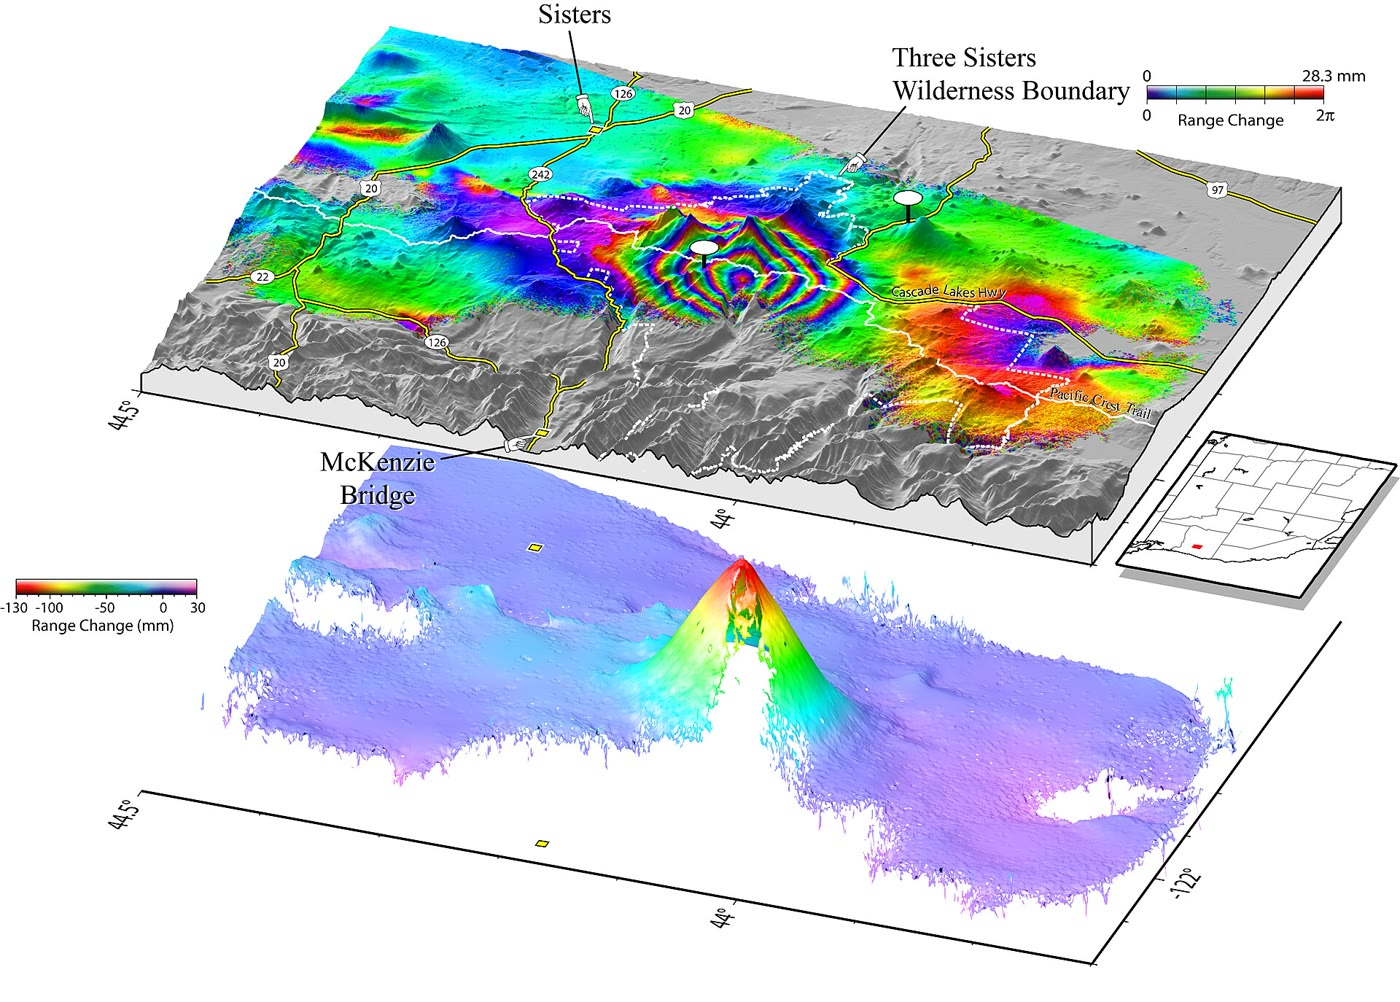
\includegraphics[width=0.86\linewidth]{images/book5/b3-three-sisters-insar.jpg}
\par\smallskip{\small Boven het \omterm{def:b3:remote-sensing-gis:insar}{interferogram} van het vulkanische centrum
Three Sisters, Oregon, 1995--2001, over het reliëf gelegd: elke cyclus van
kleuren is \qty{28.3}{mm} verandering van afstand, en de schietschijf van ringen in het
midden markeert de opheffing. Onder dezelfde gegevens, ontvouwen en getekend als een
reliëf: de afstand verkort met tot \qty{130}{mm} in het midden. U.S.
Geological Survey (Wicks en anderen, 2002), publiek
domein.}\label{fig:b3:remote-sensing-gis:three-sisters}
\end{omfigure}
% ledger: photo:b3-three-sisters-insar, usgs:insar-fs

\begin{inthelab}[Een grondstation]
\begin{minipage}[t]{0.55\linewidth}\vspace{0pt}
Een beeldvormende satelliet legt veel meer vast dan hij kan verzenden terwijl hij
het gebied passeert dat hij in beeld brengt. De radar van een Sentinel-1-satelliet kan beelden
maken tot een half uur per baan en slaat de gegevens aan boord op, tot
1410 gigabit; hij zendt ze uit via twee kanalen van 260 megabit per
seconde elk, zodat een volle opslag ongeveer 45 minuten nodig heeft om leeg te raken. Een grondstation
ontvangt ze: wanneer de satelliet boven de horizon komt, draait de schotel
zich om hem aan te wijzen, volgt hem over de hemel en laat hem los als hij ondergaat,
terwijl de operators controleren of de datastroom compleet aankomt. De gegevens gaan daarna
naar een verwerkingscentrum, waar de ruwe echo's beelden worden.
\end{minipage}\hfill
\begin{minipage}[t]{0.42\linewidth}\vspace{0pt}
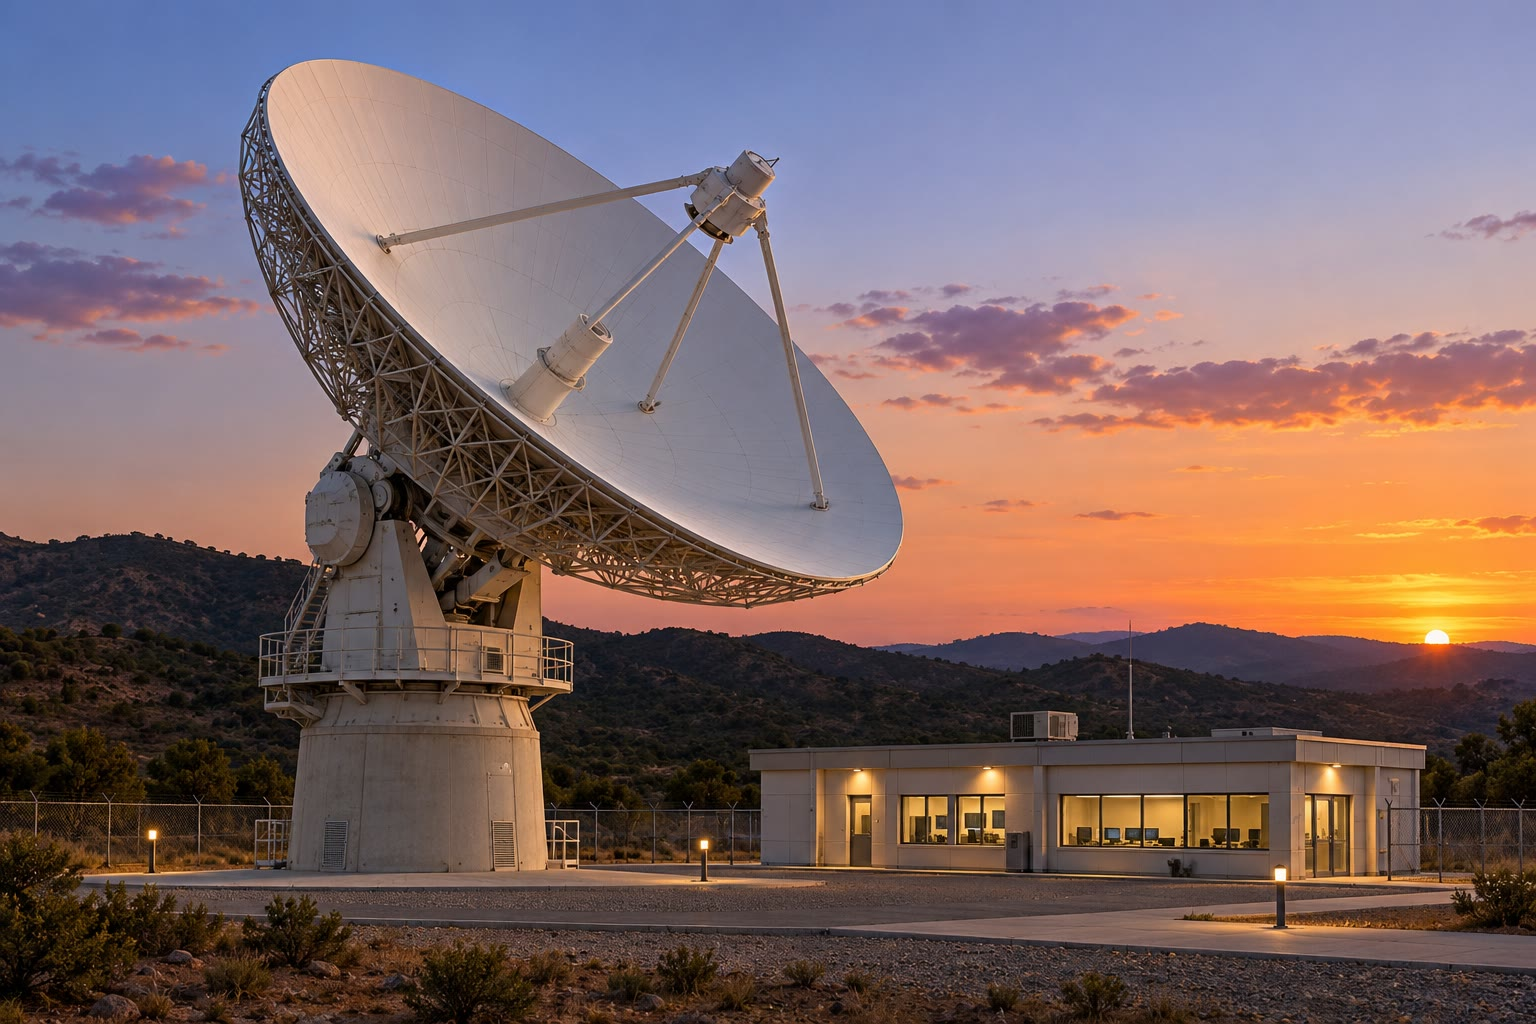
\includegraphics[width=\linewidth]{images/book5/ai/b3-ground-station.jpg}

{\scriptsize Een satellietgrondstation bij zonsondergang: een grote volgschotel en
het bedieningsgebouw (Door AI gegenereerde illustratie.)}
\end{minipage}
\end{inthelab}
% ledger: esa:s1-downlink

\section{Geografische informatiesystemen}\label{sec:b3:remote-sensing-gis:gis}

De beelden van de satellieten, het hoogtemodel van de grond, de
geologische kaart, de putten en de wegen zijn lagen van één geografisch
informatiesysteem, dat ze opslaat in een gemeenschappelijk coördinatenstelsel en
ermee rekent.

\begin{definition}[Rastergegevens en vectorgegevens]\label{def:b3:remote-sensing-gis:data-models}
\emph{Rastergegevens}\index{rastergegevens} beschrijven een laag door een rooster van
cellen, elk met één waarde: een reflectie, een hoogte, een klasse.
\emph{Vectorgegevens}\index{vectorgegevens (GIS)} beschrijven ze door punten, lijnen
en vlakken die worden gegeven door de coördinaten van hun hoekpunten, elk met een
rij attributen in een tabel.
\end{definition}

\begin{omfigure}
\centering
\begin{tikzpicture}[x=0.5cm, y=0.5cm, font=\scriptsize]
\begin{scope}
\draw[black!40] (0,0) rectangle (10,7);
\fill[omSea!50, draw=omDef, thick] (3,4.5) ellipse (1.8 and 1.2);
\draw[omDef, very thick] (4.8,4.5) -- (7,3.5) -- (10,2);
\fill[red!70!black] (7,5.5) circle (0.14); \fill[red!70!black] (2,1.5) circle (0.14);
\node[anchor=south] at (5,7.1) {vector};
\node at (3,4.5) {meer};
\node[anchor=south west] at (7.1,5.6) {put 1};
\node[anchor=south west] at (2.1,1.6) {put 2};
\node[anchor=north east] at (9.9,2.2) {rivier};
\end{scope}
\begin{scope}[xshift=6.5cm]
\foreach \i/\j in {1/4,2/4,3/4,4/4,2/3,3/3,2/5,3/5} {\fill[omSea!50] (\i,\j) rectangle ++(1,1);}
\foreach \i/\j in {5/4,6/3,7/3,8/2,9/2} {\fill[omDef!70] (\i,\j) rectangle ++(1,1);}
\foreach \i/\j in {7/5,2/1} {\fill[red!70!black] (\i,\j) rectangle ++(1,1);}
\draw[black!30, step=1] (0,0) grid (10,7);
\draw[black!40] (0,0) rectangle (10,7);
\node[anchor=south] at (5,7.1) {raster};
\end{scope}
\end{tikzpicture}
\par\smallskip{\small Dezelfde kaart als vectorgegevens (links: een vlak, een lijn
en twee punten, exact in positie, elk met zijn attributen) en als \omterm{def:b3:remote-sensing-gis:data-models}{rastergegevens}
(rechts: één waarde per cel, het meer door de cellen waarvan het middelpunt erin ligt,
de rivier en de putten door de cellen die ze kruisen). Een raster is makkelijk
te rekenen, cel voor cel; een vectorlaag behoudt vormen en topologie op
elke schaal.}\label{fig:b3:remote-sensing-gis:raster-vector}
\end{omfigure}

\begin{definition}[Georeferentie]\label{def:b3:remote-sensing-gis:georef}
\emph{Georeferentie}\index{georeferentie} is de toekenning van kaartcoördinaten
in een vastgelegde projectie aan elke pixel van een beeld of elk
hoekpunt van een tekening, meestal door een transformatie af te stemmen op grondcontrolepunten
waarvan de posities in beide stelsels bekend zijn.
\end{definition}

Voor een noord-boven raster in een geprojecteerd kader is de transformatie affien:
de cel in kolom $i$ en rij $j$ heeft haar hoekpunt bij $E = E_0 + i\,\Delta$,
$N = N_0 - j\,\Delta$, met $\Delta$ de celgrootte. Een satellietbeeld wordt
eerst geherbemonsterd naar zo'n rooster; lagen in verschillende projecties worden
samengebracht in één projectie voordat ze worden gecombineerd.

\begin{method}[Helling, aspect en reliëfschaduw uit een digitaal hoogtemodel]\label{met:b3:remote-sensing-gis:slope}
Op een rooster van hoogten $z_{i,j}$ met roosterafstand $\Delta$ ($i$ oostwaarts, $j$
noordwaarts), schat de gradiënt met centrale differenties,
\[
\frac{\partial z}{\partial x} \approx \frac{z_{i+1,j} - z_{i-1,j}}{2\Delta} ,
\qquad
\frac{\partial z}{\partial y} \approx \frac{z_{i,j+1} - z_{i,j-1}}{2\Delta} .
\]
De \emph{helling} is $S = \arctan|\nabla z|$; het \emph{aspect} is de
azimut van de steilste daling, de richting van $-\nabla z$, $A =
\operatorname{atan2}(-\partial z/\partial x, -\partial z/\partial y)$
gemeten met de klok mee vanaf het noorden. De \emph{reliëfschaduw} voor licht uit de
azimut $A_0$ bij de zenithoek $Z$ is $\cos Z\cos S + \sin Z\sin S
\cos(A_0 - A)$, de cosinus van de hoek tussen het licht en de normaal
op het grondoppervlak, op nul gezet waar die negatief is.
\end{method}

De centrale differentie is exact voor een vlak en heeft anders een fout van
$\Delta^2 z'''/6$ anders; de reliëfschaduw van de Varden Hills uit
Boek~3 is zo berekend, belicht vanuit het noordwesten. Afgeleiden
versterken de fouten van het rooster: een model met sprongen tussen zijn rijen toont
ze als strepen in zijn hellingkaart.

\begin{definition}[Kaartalgebra]\label{def:b3:remote-sensing-gis:map-algebra}
\emph{Kaartalgebra}\index{kaartalgebra} is de berekening van een nieuwe rasterlaag
cel voor cel uit een of meer lagen van hetzelfde rooster: door rekenkunde
(de NDVI uit twee banden), door vergelijking (de cellen die steiler zijn dan
\ang{15}), door logische bewerkingen (en, of, niet), of uit de omgeving
van de cel (de helling).
\end{definition}

\begin{definition}[Buffer en overlay]\label{def:b3:remote-sensing-gis:operations}
De \emph{buffer}\index{buffer (GIS)} van een object op afstand $d$ is
het gebied van de kaart binnen $d$ ervan. Een
\emph{overlay}\index{overlay (GIS)} combineert twee of meer lagen van het
zelfde gebied tot één, waarbij elke plek van het resultaat de attributen van
alle lagen draagt; de selectie van de plekken die aan meerdere voorwaarden tegelijk voldoen
is de meest voorkomende toepassing.
\end{definition}

\begin{omfigure}
\centering
\begin{tikzpicture}
\begin{groupplot}[group style={group size=2 by 2, horizontal sep=2.0cm, vertical sep=1.5cm},
  width=0.43\linewidth, axis equal image, enlargelimits=false,
  xmin=0, xmax=10, ymin=0, ymax=8,
  tick label style={font=\scriptsize}, label style={font=\small}, title style={font=\small}]
\nextgroupplot[title={(a) helling (graden)}, ylabel={noord (km)}, colormap/viridis,
  point meta min=0, point meta max=24, colorbar right,
  colorbar style={width=0.18cm, ytick={0,5,10,15,20}, tick label style={font=\tiny}, axis equal=false}]
\addplot[matrix plot*, mesh/cols=101, point meta=explicit] table[x=x, y=y, meta=slope] {figdata/out/bachelor-3-varden_gis-grid.dat};
\addplot[white, thick] table {figdata/out/shared-region-river.dat};
\nextgroupplot[title={(b) expositie},
  colormap={aspect}{rgb255=(220,20,30) rgb255=(240,200,0) rgb255=(30,170,60) rgb255=(30,90,220) rgb255=(220,20,30)},
  point meta min=0, point meta max=360, colorbar right,
  colorbar style={width=0.18cm, ytick={0,90,180,270,360}, yticklabels={N,O,Z,W,N}, tick label style={font=\tiny}, axis equal=false}]
\addplot[matrix plot*, mesh/cols=101, point meta=explicit] table[x=x, y=y, meta=aspect] {figdata/out/bachelor-3-varden_gis-grid.dat};
\addplot[black, thick] table {figdata/out/shared-region-river.dat};
\nextgroupplot[title={(c) twee lagen}, xlabel={oost (km)}, ylabel={noord (km)},
  colormap={lay}{rgb255=(245,245,245) rgb255=(150,150,150) rgb255=(225,195,140) rgb255=(120,70,20)},
  colormap access=piecewise constant, point meta min=-0.5, point meta max=3.5,
  legend columns=2, legend style={font=\tiny, at={(0.5,-0.3)}, anchor=north, /tikz/every even column/.append style={column sep=4pt}}]
\addplot[matrix plot*, mesh/cols=101, point meta=explicit, forget plot] table[x=x, y=y, meta=layers] {figdata/out/bachelor-3-varden_gis-grid.dat};
\addplot[omDef, thick, forget plot] table {figdata/out/shared-region-river.dat};
\addlegendimage{area legend, fill={rgb,255:red,150;green,150;blue,150}, draw=black!40}
\addlegendentry{steiler dan \ang{15}}
\addlegendimage{area legend, fill={rgb,255:red,225;green,195;blue,140}, draw=black!40}
\addlegendentry{schalie}
\addlegendimage{area legend, fill={rgb,255:red,120;green,70;blue,20}, draw=black!40}
\addlegendentry{beide}
\nextgroupplot[title={(d) de overlay}, xlabel={oost (km)},
  colormap={cls}{rgb255=(245,245,245) rgb255=(225,195,140) rgb255=(190,150,90) rgb255=(200,20,30)},
  colormap access=piecewise constant, point meta min=-0.5, point meta max=3.5,
  legend columns=2, legend style={font=\tiny, at={(0.5,-0.3)}, anchor=north, /tikz/every even column/.append style={column sep=4pt}}]
\addplot[matrix plot*, mesh/cols=101, point meta=explicit, forget plot] table[x=x, y=y, meta=class] {figdata/out/bachelor-3-varden_gis-grid.dat};
\addplot[omDef, thick, forget plot] table {figdata/out/shared-region-river.dat};
\addplot[black, thin, dashed, unbounded coords=jump] table[x=x, y=y] {figdata/out/bachelor-3-varden_gis-buffer.dat};
\addlegendentry{\qty{1}{km} buffer}
\addlegendimage{area legend, fill={rgb,255:red,225;green,195;blue,140}, draw=black!40}
\addlegendentry{schalie}
\addlegendimage{area legend, fill={rgb,255:red,190;green,150;blue,90}, draw=black!40}
\addlegendentry{schalie in buffer}
\addlegendimage{area legend, fill={rgb,255:red,200;green,20;blue,30}, draw=black!40}
\addlegendentry{geselecteerd}
\end{groupplot}
\end{tikzpicture}
\par\smallskip{\small Een GIS-sessie op de Varden Hills, op basis van hun hoogtemodel
op een rooster van \qty{100}{m}. (a)~De helling, tot \ang{23} op de
dalwanden; (b)~het aspect, de richting waarin de grond is gericht, de twee
oevers van de rivier die naar elkaar gericht zijn; (c)~twee lagen, de cellen steiler dan \ang{15}
en de ontsluiting van de Jurassische schalie; (d)~hun \omterm{def:b3:remote-sensing-gis:operations}{overlay} met de
\omterm{def:b3:remote-sensing-gis:operations}{buffer} van \qty{1}{km} rond de rivier (gestreept): de \qty{0.32}{km^2} aan steile
schalie boven de rivier, een eerste zeef voor terrein dat
kan afschuiven.}\label{fig:b3:remote-sensing-gis:varden}
\end{omfigure}

De figuur hierboven doorloopt de hele keten: \omterm{def:b3:remote-sensing-gis:map-algebra}{kaartalgebra} op het hoogterooster
levert de helling en het aspect; een vergelijking maakt van de helling een laag
van steile cellen; de geologische kaart levert de schalie; de \omterm{def:b3:remote-sensing-gis:operations}{buffer} van de
rivier levert een derde laag; hun doorsnede, een \omterm{def:b3:remote-sensing-gis:operations}{overlay} met de logische
\emph{en}, laat 32 cellen van de 8181 over. Het antwoord is slechts zo goed als de
lagen: op een grover rooster vallen de hellingen zachter uit en passeren er minder cellen.

\begin{definition}[Gesuperviseerde classificatie; verwarringsmatrix]\label{def:b3:remote-sensing-gis:classification}
Een \emph{gesuperviseerde classificatie}\index{gesuperviseerde classificatie}
wijst elke pixel van een beeld toe aan een van een reeks klassen, op basis van regels of
statistieken die zijn geleerd op trainingspixels waarvan de klasse op het terrein bekend is.
Zijn \emph{verwarringsmatrix}\index{verwarringsmatrix} telt, voor een afzonderlijke
reeks referentiepixels, hoeveel pixels van elke werkelijke klasse aan elke
klasse zijn toegewezen: $n_{ij}$ pixels die als $i$ zijn geclassificeerd, horen in werkelijkheid bij $j$.
\end{definition}

De diagonaal bevat de pixels die goed zijn geclassificeerd. Met $N$ referentiepixels,
is de \emph{totale nauwkeurigheid} $\sum_i n_{ii}/N$. De \emph{gebruikersnauwkeurigheid}
van een klasse, $n_{ii}$ gedeeld door het rijtotaal, is de kans dat een
pixel die de kaart $i$ noemt, werkelijk $i$ is; de \emph{producentennauwkeurigheid}, $n_{ii}$
gedeeld door het kolomtotaal, is de kans dat een werkelijke $i$ als $i$ is in kaart gebracht. De
\emph{kappa}-coëfficiënt vergelijkt de totale nauwkeurigheid $p_o$ met de
nauwkeurigheid $p_e = \sum_i (\text{rij}_i)(\text{kolom}_i)/N^2$ die willekeurige
toewijzing met dezelfde totalen zou bereiken: $\kappa = (p_o - p_e)/(1 -
p_e)$.

\begin{center}
\small
\begin{tabular}{l|ccc|c}
\hline
geclassificeerd \textbackslash{} referentie & water & bos & kaal gesteente & totaal \\
\hline
water & 45 & 2 & 0 & 47 \\
bos & 3 & 38 & 7 & 48 \\
kaal gesteente & 0 & 5 & 30 & 35 \\
\hline
totaal & 48 & 45 & 37 & 130 \\
\hline
\end{tabular}
\end{center}

In dit verzonnen voorbeeld zijn 113 van de 130 pixels goed, een totale nauwkeurigheid
van \qty{86.9}{\percent}. Bos heeft een gebruikersnauwkeurigheid van
$38/48 = \qty{79}{\percent}$ maar een producentennauwkeurigheid van $38/45 =
\qty{84}{\percent}$: zeven pixels van kaal gesteente, misschien in de schaduw,
werden als bos aangeduid. Willekeurige toewijzing zou $p_e = 0.338$ bereiken, en $\kappa =
0.80$.

\section{Oefeningen}

\begin{exercise}[$\star$]\label{exo:b3:remote-sensing-gis:1}
Een veld heeft reflectanties van 0.06 in de rode band en 0.42 in de
nabij-infraroodband van een beeldsensor; een naastgelegen geploegd veld 0.21 en
0.28. Bereken de NDVI van beide en geef aan wat elke waarde suggereert.
\end{exercise}

\begin{exercise}[$\star$]\label{exo:b3:remote-sensing-gis:2}
De Landsat~8-beeldsensor dekt een strook \qty{185}{km} breed met \qty{30}{m}
pixels en zijn panchromatische band met \qty{15}{m} pixels. (a)~Hoeveel
pixels bevat een lijn dwars over de strook in elk geval? (b)~Hoeveel niveaus
geven 12 bits, en 8 bits? (c)~Wat is de \omterm{def:b3:remote-sensing-gis:resolutions}{terugkeertijd} van Landsat~8
alleen, en van Landsat 8 en 9 samen?
\end{exercise}

\begin{exercise}[$\star$]\label{exo:b3:remote-sensing-gis:3}
(a)~Op een Sentinel-1-interferogram ($\lambda = \qty{5.55}{cm}$) van een
zakkend bekken scheiden zes interferentiebanden de stabiele rand van het midden.
Wat is de verandering van de \omterm{def:b3:remote-sensing-gis:insar}{zichtlijn} in het midden? (b)~Wat zou één
interferentieband voor een oudere satelliet met golflengte \qty{5.66}{cm} zijn?
\end{exercise}

\begin{exercise}[$\star$]\label{exo:b3:remote-sensing-gis:4}
Een laseraltimeter bevindt zich \qty{500}{km} boven het aardoppervlak. (a)~Hoe lang
doet een lichtpuls erover om terug te keren? (b)~Als de aankomsttijd van elk foton tot
\qty{800}{ps} nauwkeurig is bepaald, hoe precies is één afstandsbepaling?
\end{exercise}

\begin{exercise}[$\star\star$]\label{exo:b3:remote-sensing-gis:5}
Een pixel van Landsat~8, band~10 (neem $\lambda = \qty{10.9}{\micro\metre}$)
heeft, na \omterm{def:b3:remote-sensing-gis:atm-correction}{atmosferische correctie}, een spectrale radiantie van
\qty{9.0}{W.m^{-2}.sr^{-1}.\micro\metre^{-1}}. (a)~Bereken de
\omterm{def:b3:remote-sensing-gis:brightness}{helderheidstemperatuur}. (b)~Het oppervlak is een grasveld met emissiviteit 0.98: wat is
de kinetische temperatuur?
\end{exercise}

\begin{exercise}[$\star\star$]\label{exo:b3:remote-sensing-gis:6}
De Sentinel-1-radar vliegt op \qty{693}{km} hoogte met een antenne van \qty{12.3}{m}
lang bij $\lambda = \qty{5.55}{cm}$. (a)~Negeer de kromming van de
Aarde, bereken de schuine afstand tot een punt dat onder een invalshoek van
\ang{35} wordt gezien. (b)~Welke azimutresolutie zou een echte antenne van die lengte
daar geven, en wat levert de synthetische apertuur op? (c)~Hoe lang is de
synthetische apertuur?
\end{exercise}

\begin{exercise}[$\star\star$]\label{exo:b3:remote-sensing-gis:7}
Een venster van $3\times3$ cellen uit een digitaal hoogtemodel met \qty{30}{m} cellen
leest, met het noorden bovenaan,
\[
\begin{matrix} 412 & 418 & 425 \\ 405 & 410 & 418 \\ 398 & 401 & 409 \end{matrix}
\qquad (\unit{m}).
\]
Bereken met centrale differenties in de middencel de helling, het aspect
en het schaduwreliëf voor licht uit het noordwesten, \ang{45} boven de
horizon.
\end{exercise}

\begin{exercise}[$\star\star$]\label{exo:b3:remote-sensing-gis:8}
Een landbedekkingskaart wordt gecontroleerd aan de hand van 160 referentiepixels (rijen: de kaart;
kolommen: de werkelijkheid; klassen water, bos, gewassen, stad):
\[
\begin{pmatrix} 48 & 3 & 1 & 0 \\ 4 & 37 & 6 & 1 \\ 2 & 5 & 29 & 2 \\ 0 & 1 & 2 & 19 \end{pmatrix} .
\]
Bereken de totale nauwkeurigheid, de gebruikersnauwkeurigheid en de producentennauwkeurigheid van elke
klasse, en kappa. Welke klasse wordt het vaakst gemist?
\end{exercise}

\begin{exercise}[$\star\star$]\label{exo:b3:remote-sensing-gis:9}
Een thermische pixel van \qty{100}{m} bevat een verse lavastroom van \qty{1443}{K}
die \qty{4}{\percent} ervan bedekt; de rest is grond van \qty{290}{K}; beschouw
beide als zwarte lichamen. (a)~Bereken de \omterm{def:b3:remote-sensing-gis:brightness}{helderheidstemperatuur} van de pixel
bij \qty{10.9}{\micro\metre} en vergelijk die met de gemiddelde temperatuur.
(b)~Bereken de verhouding van de zwartlichaamsstraling van de lava en de
grond bij \qty{2.2}{\micro\metre}, en de \omterm{def:b3:remote-sensing-gis:brightness}{helderheidstemperatuur} van de
pixel daar. Welke band detecteert de lava beter?
\end{exercise}

\begin{exercise}[$\star\star\star$]\label{exo:b3:remote-sensing-gis:10}
Twee interferogrammen van dezelfde vervorming worden gemaakt uit twee passages, één
met de satelliet ten oosten van het aardoppervlak en één met de satelliet ten westen ervan,
beide bij een invalshoek van \ang{35}. Op één punt verkort de
\omterm{def:b3:remote-sensing-gis:insar}{zichtlijn} met \qty{64}{mm} bij de eerste en \qty{38}{mm} bij de
tweede. Neem aan dat er geen beweging in noord--zuidrichting is en bereken de verticale en de
oostwaartse verplaatsing. Waarom is één passage niet genoeg?
\end{exercise}

\begin{exercise}[$\star\star\star$]\label{exo:b3:remote-sensing-gis:11}
\omterm{def:b3:remote-sensing-gis:insar}{Fase-ontvouwing} mislukt waar de fase met meer dan $\pi$ springt tussen
naburige pixels. (a)~Toon aan dat de \omterm{def:b3:remote-sensing-gis:insar}{zichtlijn} van de ene pixel naar de volgende moet
veranderen met minder dan $\lambda/4$, \qty{13.9}{mm} voor
Sentinel-1. (b)~Voor een Mogi-bron op $z_0 = \qty{4}{km}$ met $\Delta V =
\qty{e7}{m^3}$ en $\nu = 0.25$, verticaal gezien, toon aan dat de steilste
gradiënt van $u_z$ ligt bij $r = z_0/2$ en bereken die. (c)~Wat is de
grootste pixelgrootte waarbij de interferentiestrepen nog oplosbaar zijn?
\end{exercise}

\begin{exercise}[$\star\star\star$]\label{exo:b3:remote-sensing-gis:12}
(a)~Toon aan dat de NDVI ligt tussen $-1$ en $+1$ voor niet-negatieve
reflectanties, en dat hij onveranderd blijft wanneer beide reflectanties
met dezelfde factor worden vermenigvuldigd. (b)~Gras heeft reflectanties van 0.051 (rood)
en 0.502 (nabij-infrarood). Een niet-gecorrigeerd beeld voegt een padstraling toe
gelijk aan 0.03 in het rood en 0.01 in het nabij-infrarood. Bereken de
NDVI met en zonder die padstraling. (c)~Wat betekent dat voor een kaart van de NDVI
gemaakt uit niet-gecorrigeerde beelden op een dunstige dag?
\end{exercise}

\section{Probleem: Een zwellende flank van Mount Halvren}

\begin{problem}[{Weekendprobleem --- vegetatie, warmte en een radar
interferogram op een verzonnen vulkaan}]
\label{pb:b3:remote-sensing-gis:1}
Mount Halvren, een verzonnen vulkaan, heeft in 1890, 1960
en 2005 lavastromen uitgestoten op zijn beboste flanken. Op de top stoomt een fumarolenveld.
Satellietgegevens van een recent jaar staan hieronder.

\medskip\noindent\textbf{Deel I --- Vegetatie op de lavastromen.} Gecorrigeerde
reflectanties in de rode en nabij-infrarode banden:
\begin{center}
\small
\begin{tabular}{lcccc}
\hline
oppervlak & bos & lavastroom van 1890 & lavastroom van 1960 & lavastroom van 2005 \\
\hline
rood & 0.04 & 0.07 & 0.11 & 0.12 \\
nabij-infrarood & 0.38 & 0.30 & 0.21 & 0.14 \\
\hline
\end{tabular}
\end{center}
\begin{enumerate}
\item Bereken de NDVI van de vier oppervlakken.
\item Rangschik de lavastromen naar het herstel van hun vegetatie. Is de rangorde
  die van hun ouderdom?
\item Waarom is de NDVI van de lavastroom van 2005 niet nul, hoewel er vrijwel
  niets op groeit?
\item Waarom is de NDVI betrouwbaarder dan de nabij-infraroodreflectantie
  alleen op de steile, ongelijk belichte flanken van een vulkaan?
\end{enumerate}

\medskip\noindent\textbf{Deel II --- Het fumarolenveld.} In de thermische
band (neem $\lambda = \qty{10.9}{\micro\metre}$) de gecorrigeerde straling van
een pixel van \qty{100}{m} op het topplateau, uit de buurt van de fumarolen, is
\qty{8.40}{W.m^{-2}.sr^{-1}.\micro\metre^{-1}}, en die van de pixel boven
het fumarolenveld \qty{9.95}{W.m^{-2}.sr^{-1}.\micro\metre^{-1}}.
\begin{enumerate}[resume]
\item Bereken de helderheidstemperaturen van de twee pixels.
\item Het gesteente van het plateau heeft een emissiviteit van 0.97. Wat is de kinetische
  temperatuur?
\item De fumaroleopeningen en de warme grond eromheen zijn op
  \qty{370}{K}. Beschouw ze en de rest van de pixel als zwarte lichamen,
  met de rest op de straling van het plateau, welk deel van de pixel ze bedekken,
  en welk oppervlak?
\item Waarom blijft de oppervlaktegewogen gemiddelde temperatuur van de pixel
  achter bij de \omterm{def:b3:remote-sensing-gis:brightness}{helderheidstemperatuur}?
\end{enumerate}

\medskip\noindent\textbf{Deel III --- Het interferogram.} Twee Sentinel-1
beelden ($\lambda = \qty{5.55}{cm}$, invalshoek \ang{35}, satelliet ten
oosten), met 48 dagen ertussen genomen, tonen een concentrisch patroon op de oostflank.
Van een stabiel gebied tot het centrum van het patroon telt men vijf volledige strepen en
vier tiende van een zesde, alle in de zin van beweging naar de
satelliet toe.
\begin{enumerate}[resume]
\item Waarom moeten twee beelden vanuit bijna dezelfde positie worden genomen, en
  hoeveel baancycli van één satelliet ze van elkaar scheiden?
\item Bereken de verandering van de \omterm{def:b3:remote-sensing-gis:insar}{zichtlijn} in het centrum.
\item In het centrum beweegt de grond alleen verticaal. Bereken de opheffing
  daar.
\item Verklaar waarom het patroon niet cirkelvormig is, en aan welke kant, oost of
  west, de strepen het dichtst op elkaar liggen.
\item Langs de noord--zuidlijn door het centrum daalt de verandering van de
  \omterm{def:b3:remote-sensing-gis:insar}{zichtlijn} tot de helft van haar centrale waarde op \qty{3.4}{km} van het
  centrum. Waarom gebruikt men die lijn, en welke diepte volgt er dan voor
  een Mogi-bron?
\item Hoeveel strepen liggen er tussen het centrum en dat punt op halve hoogte?
\item Waterdamp in de lucht kan de radargolven op de twee data verschillend vertragen
  en daarmee eigen strepen veroorzaken. Hoe zou een tweede \omterm{def:b3:remote-sensing-gis:insar}{interferogram},
  van een ander paar data, helpen de twee van elkaar te onderscheiden?
\end{enumerate}

\medskip\noindent\textbf{Deel IV --- Het volume.} Neem $\nu = 0.25$.
\begin{enumerate}[resume]
\item Bereken uit $u_z(0) = (1 - \nu)\Delta V/(\pi z_0^2)$ de volumeverandering van de
  bron.
\item Geef dat als een gemiddelde snelheid per dag en per jaar over de 48 dagen.
\item Bereken de grootste horizontale verplaatsing en waar die optreedt.
\item Als het reservoir een bol met straal $z_0/3$ zou zijn, hoe groot zou het
  volume zijn, en welk deel daarvan vertegenwoordigt de verandering?
\item De eindige omvang van een bol met straal $z_0/3$ verandert de opheffing met
  ongeveer \qty{3}{\percent}. Verandert dat het antwoord op vraag~16
  merkbaar, gezien de precisie van het tellen van de strepen?
\item Welke andere waarneming, uit delen I en II of van het terrein,
  zou de interpretatie van een zich vullend reservoir ondersteunen?
\item Geef de volumeverandering van het reservoir onder Mount Halvren,
  in miljoen kubieke meter, met twee significante cijfers.
\end{enumerate}
\end{problem}
% ledger: nasa:ndvi, esa:s1-sar, esa:s1-orbit, esa:s1-iw, dmodels:mogi, dmodels:mogi-radial, const:h, const:c, const:kB
